
%%%%%
%%%%% DO NOT EDIT THIS FILE
%%%%%



\documentclass[12pt,a4paper,fleqn]{report}

%%% packages for mathematical typesetting
\usepackage{amsmath}
\usepackage{amssymb}
\usepackage{times}
\usepackage{bm}
%\usepackage{mathtools}
%\usepackage{nicefrac}
%\usepackage{latexsym}

%%% packages for including figures and subfigures
\usepackage{graphicx}
\usepackage[font=footnotesize,labelformat=empty]{subfig}

%%% package for nicer table layout
\usepackage{booktabs}
\usepackage{colortbl}

%%% package for color mangement
\usepackage[svgnames]{xcolor}

%%% package for page headings and footers
\usepackage{fancyhdr}

%%% package for hyperlinks
\usepackage{hyperref}
\hypersetup{%
  colorlinks=true,
  urlcolor=DarkGreen,
  citecolor=green,
  bookmarks=false}


\usepackage[noend]{algpseudocode}
\algrenewcommand\algorithmicdo{}
\algrenewcommand\algorithmicthen{}
\algrenewcommand{\algorithmiccomment}[1]{// #1}
\makeatletter
\newcommand{\StatexIndent}[1][3]{%
  \setlength\@tempdima{\algorithmicindent}%
  \Statex\hskip\dimexpr#1\@tempdima\relax}
\makeatother


\usepackage{fancyvrb} 
\usepackage{listings}
% Python style / environment for highlighting in "figures"
\lstdefinestyle{pythonstyle}{%
  language=Python,
  tabsize=4,
  backgroundcolor=\color{Gray!10},
  basicstyle=\ttfamily\scriptsize,
  stringstyle=\color{ForestGreen},
  keywordstyle=\color{BlueViolet},
  commentstyle=\itshape\color{DarkRed!90},
  identifierstyle=,
  emphstyle=\color{Blue},
  frame=lines,	
  showstringspaces=false,
  morekeywords={range, len, self, lambda, from, import, as, False, True, enumerate, map, list, set, float, int, min, max, with}
  fancyvrb=true,
}
\lstnewenvironment{python}[1][]{\lstset{style=pythonstyle,#1}}{}





\graphicspath{{./Figures/}, {./Images/}}



%%% text highlighting
\newcommand{\keyword}[1]{\emph{\texttt{\color{blue}#1}}}
\newcommand{\alert}[1]{\emph{\texttt{\color{red}#1}}}


%%% sets
\newcommand{\set}[1]{#1}

%%% vectors, matrices, and tensors
\renewcommand{\vec}[1]{\bm{#1}}
\newcommand{\mat}[1]{\bm{#1}}
\newcommand{\ten}[1]{\bm{\mathcal{#1}}}

%%% trace, rank, and diagonal
\newcommand{\tr}[1]{\operatorname{tr} \bigl [ #1 \bigr ]}
\newcommand{\TR}[1]{\operatorname{tr} \Bigl [ #1 \Bigr ]}
\newcommand{\rk}[1]{\operatorname{rk} \bigl [ #1 \bigr ]}
\newcommand{\RK}[1]{\operatorname{rk} \Bigl [ #1 \Bigr ]}
\newcommand{\diag}[1]{\operatorname{diag} \bigl [ #1 \bigr ]}
\newcommand{\DIAG}[1]{\operatorname{diag} \Bigl [ #1 \Bigr ]}

%%% inverse and transpose
\newcommand{\inv}[1]{#1^{-1}}
\newcommand{\trn}[1]{#1^\intercal}
\newcommand{\invtrn}[1]{#1^{-\intercal}}

%%% outer product
\newcommand{\opt}[2]{#1 \trn{#2}}

%%% inner products
\newcommand{\ipt}[2]{\trn{#1} #2}
\newcommand{\iptb}[2]{\left( \ipt{#1}{#2} \right)}
\newcommand{\ip}[2]{\langle #1, #2 \rangle}
\newcommand{\Ip}[2]{\bigl \langle #1, #2 \bigr \rangle}
\newcommand{\ipa}[2]{\langle #1, #2 \rangle}
\newcommand{\Ipa}[2]{\bigl \langle #1, #2 \bigr \rangle}
\newcommand{\dsq}[2]{\bigl \lVert #1 - #2 \bigr \rVert^2}
\newcommand{\nrm}[1]{\bigl \lVert #1 \bigr \rVert^2}
\newcommand{\sdsq}[2]{\lVert #1 - #2 \rVert^2}
\newcommand{\snrm}[1]{\lVert #1 \rVert^2}


\newcommand{\st}{\operatorname{s.\!t.}}
\newcommand{\amin}[1]{\operatorname*{argmin}_{#1}}
\newcommand{\amax}[1]{\operatorname*{argmax}_{#1}}

\newcommand{\submax}[1]{#1_{\text{max}}}

\newcommand{\ci}{\perp\!\!\!\perp}
\newcommand{\prob}[1]{p\bigl( #1 \bigr)}
\newcommand{\cprob}[2]{p\bigl( #1 \bigm| #2 \bigr)}

%%% horizontal and vertical dash
\newcommand{\hdash}{\operatorname{\,{}---{}\,}}
\renewcommand{\vdash}{\arrowvert}





\pagestyle{fancy}
\lhead{\emph{Pattern Recognition (2)}}
\rhead{\emph{Summer Term 2021}}
\cfoot{}

\frenchspacing

\setlength{\parskip}{1ex plus0.5ex minus0.5ex}

\setlength{\headheight}{15pt}

\def\thesection{\arabic{section}.}
\setlength{\parindent}{0pt}

\renewcommand{\familydefault}{\sfdefault}





\begin{document}

\subsection*{exercise 3}
\textbf{simple proofs, fastmap, and Hopfield nets}
\vspace{1cm}

\subsection*{solutions due}
until \textbf{May 30, 2021} at \textbf{23:59} via \textbf{email}
\vspace{1cm}

\vfill


\subsection*{students handing in this solution set}

\begin{tabular*}{\textwidth}{l@{\extracolsep{\fill}}lll}
  \toprule
  last name & first name & student ID & enrolled with \\
  \midrule
  \midrule
  Nikolskyy
  & Oleksander
  & TODO
  & TODO
  \\
  Schier
  & Marie
  & TODO
  & TODO
  \\
  Doll
  & Niclas
  & 3075509
  & Uni Bonn
  \\
  Safavi
  & Arash
  & TODO
  & TODO
  \\
  Wani
  & Mohamad Saalim
  & TODO
  & TODO
  \\
  Bonani
  & Mayara Everlim
  & TODO
  & TODO
  \\
  \bottomrule
\end{tabular*}
\newpage

%%%%%
%%%%% DO NOT EDIT THE FOLLOWING
%%%%%

\subsection*{general remarks}

As you know, your instructor is an avid  proponent of open science and education. Therefore, \textbf{MATLAB implementations will not be accepted} in this course.

The goal of this exercise is to get used to scientific Python. There are numerous resources on the web related to Python programming. Numpy and Scipy are well documented and Matplotlib, too, comes with numerous tutorials. Play with the code that is provided. Most of the above tasks are trivial to solve, just look around for ideas as to how it can be done.

Remember that you have to achieve at least 50\% of the points of the exercises to be eligible to the written exam at the end of the semester. Your grades (and credits) for this course will be decided based on the exam only, but --once again-- you have to succeed in the exercises to get there.
  
Your solutions have to be \emph{satisfactory} to count as a success. Your code and results will be checked and need to be convincing.

If your solutions meets the above requirements and you can demonstrate that they work in practice, it is a \emph{satisfactory} solution.

A \emph{very good} solution (one that is rewarded full points) requires additional efforts especially w.r.t. to readability of your code. If your code is neither commented nor well structured, your solution is not good! The same holds for your discussion of your results: these should be concise and convincing and demonstrate that you understood what the respective task  was all about. Striving for very good solutions should always be your goal!
 



\subsection*{practical advice}



The problem specifications you'll find below assume that you use python / numpy / scipy for your implementations. They also assume that you have imported the following
\begin{python}
import numpy as np
import numpy.linalg as la
import matplotlib.pyplot as plt
\end{python}


\subsection*{task 3.1 [5 points] \\[1ex] whitened data is of unit covariance}

In lecture 08, we briefly looked at data pre-processing techniques such as \emph{data whitening}. Recall that, if we are given an $m \times n$ data matrix of real valued vectors
\begin{equation*}
\mat{X} = 
\begin{bmatrix}
\vdash    & \vdash    &        & \vdash \\
\vec{x}_1 & \vec{x}_2 & \cdots & \vec{x}_n \\
\vdash    & \vdash    &        & \vdash \\
\end{bmatrix}
\end{equation*}
then the process of whitening these data consists of the following three steps
\begin{enumerate}
\item compute the transformation
  \begin{equation*}
  \mat{Y} = \mat{X} \, \bigl( \mat{I} - \tfrac{1}{n} \, \opt{\vec{1}}{\vec{1}} \bigr)
  \end{equation*}
\item determine the spectral decomposition
  \begin{equation*}
  \tfrac{1}{n} \, \opt{\mat{Y}}{\mat{Y}} = \mat{U} \mat{\Lambda} \, \trn{\mat{U}}
  \end{equation*}
\item  compute the transformation
  \begin{equation*}
  \mat{Z} = \mat{U} \, \mat{\Lambda}^{-\frac{1}{2}} \trn{\mat{U}} \mat{Y}
  \end{equation*}
\end{enumerate}
Also recall that we claimed the covariance matrix of the data in $\mat{Z}$ to be the identity matrix. Your task is now to prove this claim, i.e. prove that
\begin{equation*}
\frac{1}{n} \, \opt{\mat{Z}}{\mat{Z}} = \mat{I}
\end{equation*}
(Remember that $\mat{U}$ is orthogonal and $\mat{\Lambda}$ is diagonal \ldots)
\color{blue} \\[1ex]
%%%%%
%%%%%
%%%%% enter your proof here
%%%%%
%%%%%
\begin{align*}
\opt{\mat{Z}}{\mat{Z}} 
&= (\mat{U} \mat{\Lambda}^{-\frac12} \mat{U}^T \mat{Y}) (\mat{U} \mat{\Lambda}^{-\frac12} \mat{U}^T \mat{Y})^T \\
&= \mat{U} \mat{\Lambda}^{-\frac12} \mat{U}^T (\mat{Y} \mat{Y}^T ) \mat{U} \mat{\Lambda}^{-\frac12} \mat{U}^T \\
&= \mat{U} \mat{\Lambda}^{-\frac12} \mat{U}^T (n \cdot \frac1n \mat{Y} \mat{Y}^T ) \mat{U} \mat{\Lambda}^{-\frac12} \mat{U}^T \\
&= \mat{U} \mat{\Lambda}^{-\frac12} \mat{U}^T (n \cdot \mat{U} \mat{\Lambda} \mat{U}^T ) \mat{U} \mat{\Lambda}^{-\frac12} \mat{U}^T \\
&= n \cdot \mat{U} \mat{\Lambda}^{-\frac12} \mat{U}^T \mat{U} \mat{\Lambda} \mat{U}^T \mat{U} \mat{\Lambda}^{-\frac12} \mat{U}^T \\
&= n \cdot \mat{U} \mat{\Lambda}^{-\frac12} \mat{\Lambda} \mat{\Lambda}^{-\frac12} \mat{U}^T \\
&= n \cdot \mat{U} \mat{U}^T \\
&= n \cdot \mat{I}
\end{align*}

%%%%%
%%%%%
%%%%%
%%%%%
%%%%%
\color{black}






\subsection*{task 3.2 [5 points] \\[1ex] more on idempotent matrices}

In lecture 07, we already proved that, if $\vec{u} \in \mathbb{R}^m$ is a unit vector, then the outer product matrix $\mat{P} = \opt{\vec{u}}{\vec{u}}$ is idempotent. Your task is now to establish a more general result.

Prove that, for any $\vec{u} \neq \vec{0} \in \mathbb{C}^m$, the matrix
\begin{equation*}
\mat{P} = \frac{\vec{u} \vec{u}^\dagger}{\vec{u}^\dagger \vec{u}}
\end{equation*}
is idempotent.
\color{blue} \\[1ex]
%%%%%
%%%%%
%%%%% enter your proof here
%%%%%
%%%%%
\begin{align*}
\mat{P}^2
&= \left( \frac{\vec{u} \vec{u}^\dagger}{\vec{u}^\dagger \vec{u}} \right) \left( \frac{\vec{u} \vec{u}^\dagger}{\vec{u}^\dagger \vec{u}} \right) 
= \frac{\vec{u} (\vec{u}^\dagger \vec{u}) \vec{u}^\dagger}{(\vec{u}^\dagger \vec{u})^2}
= \frac{\vec{u} \vec{u}^\dagger}{\vec{u}^\dagger \vec{u}} = \mat{P}
\end{align*}

%%%%%
%%%%%
%%%%%
%%%%%
%%%%%
\color{black}






\subsection*{task 3.3 [10 points] \\[1ex] fastmap}

In the \texttt{Data} folder for this exercise, you will find the file
\begin{quote}
    \texttt{faceMatrix.npy}
\end{quote}
which contains a data matrix $\mat{X} \in \mathbb{R}^{361 \times 2429}$ whose columns $\vec{x}_i$ represent tiny face images of size $19 \times 19$ pixels. To read this matrix into memory and check its size, you may use
\begin{python}
matX = np.load('faceMatrix.npy').astype('float')
m, n = matX.shape
print (m, n)
\end{python}
To have a look at one of the images it contains, say $\vec{x}_{15}$, you may use this
\begin{python}
vecX = matX[:,14].reshape(19,19)
plt.imshow(vecX, cmap='gray')
plt.xticks([])
plt.yticks([])
plt.show()
\end{python}
\vspace{2cm}


Having read matrix $\mat{X}$ into memory, here is what you are supposed to do:

\begin{enumerate}
\item Implement the \emph{fastmap} algorithm which we discussed in lecture 07. Recall that this algorithm involves a function \textsc{getDistantObjects}. How would you implement it in numpy / scipy?
%%%%%
%%%%%
%%%%% enter your code into the following environment
%%%%%
%%%%%
\begin{python}
# helper function to compute the squared norm of vectors
sq_norm = lambda X: (X ** 2).sum(axis=0)
# function implementing fastmap
def fastmap(
    X:np.ndarray, 
    k:int
) -> np.ndarray:
    m, n = X.shape
    # list of the computed approximations
    V = []
    # do the iterations
    for _ in range(k):
        # find the two most distant object indices
        i = np.random.choice(n, size=1)[0]
        j = sq_norm(X - X[:, i:i+1]).argmax()
        i = sq_norm(X - X[:, j:j+1]).argmax()
        j = sq_norm(X - X[:, i:i+1]).argmax()
        # approximate the major component of the current matrix X
        v = (X[:, j:j+1] - X[:, i:i+1])
        v /= la.norm(v, axis=0)
        # add the major component to the list
        V.append(v)
        # project vectors into subspace
        X = (np.eye(m) - v @ v.T) @ X
    # stack all approximations and return
    return np.concatenate(V, axis=1)
\end{python}
%%%%%
%%%%%
%%%%%
%%%%%
%%%%%

\item Run your \emph{fastmap} implementation to obtain approximations of the top $25$ principal components of the data in matrix $\mat{X}$. 
\begin{python}
# compute approximations of major components using fastmap
V = fastmap(X, k=25)
\end{python}

\item  Compute the SVD of matrix $\mat{X}$ and determine the top $25$ left singular vectors.
\begin{python}
# compute the left singular vectors of the data matrix using svd
U, _, _ = la.svd(X)
# get only the first 25 singular vectors and ignore the rest
# note that the singular values are sorted in non-increasing order
# thus the first k singular vectors are the first k major components
U = U[:, :25]
\end{python}

\item Compare your \emph{fastmap} results to your SVD results. A good idea for doing this is to visualize / plot them as tiny images; figure out how to create a plot that shows not just a single tiny image but $25$ at the same time

%%%%%
%%%%%
%%%%% enter plots here, i.e. replace "placeholder.pdf" by the name of the graphics files you created
%%%%%
%%%%%
\begin{center}
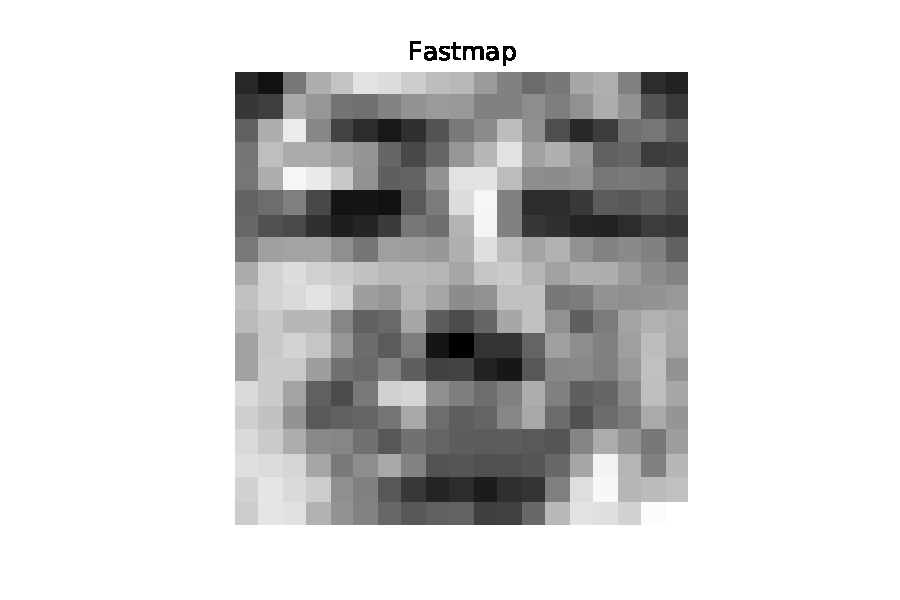
\includegraphics[width=0.45\textwidth]{Ex_03/Figures/fastmap.pdf}
\hfill
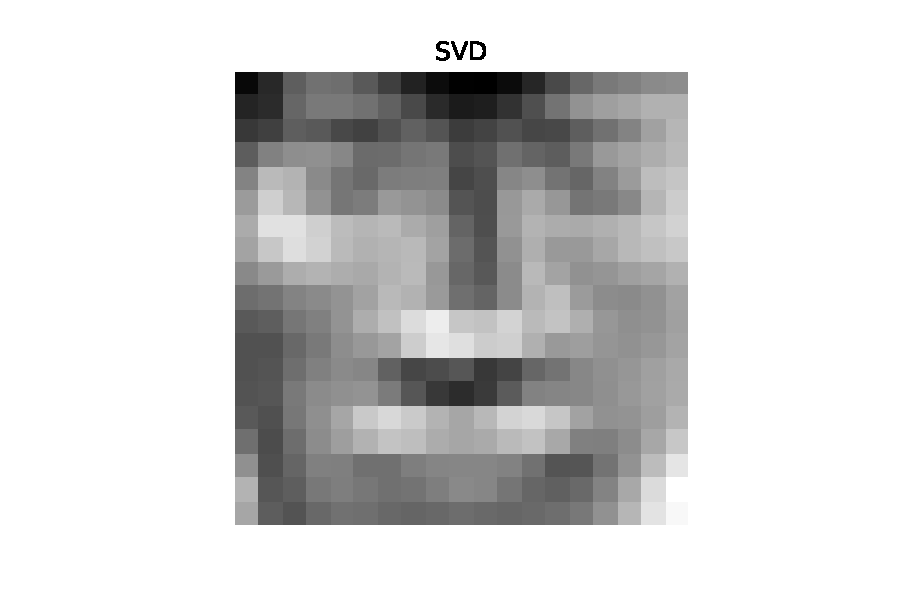
\includegraphics[width=0.45\textwidth]{Ex_03/Figures/svd.pdf}
\end{center}
%%%%%
%%%%%
%%%%%
%%%%%
%%%%%
\end{enumerate}



\subsection*{task 3.4 [10 points] \\[1ex] Hopfield nets: the $k$-rooks problem}

In lecture 10, we introduced the $k$-rooks problem and saw how to solve it using a Hopfield network. In particular, we considered the special case where $k=4$. Building on our discussion, here is what you are supposed to do in this task:

\begin{python}
# this is pretty much the exact code given in the lecture
# define the signum function
signum = lambda x: np.where(x >= 0, +1, -1)
# run the asynchronous hopfield network updates for some number of steps
def hopfield_run_async(s, W, theta, tmax=1000):
    for u in np.random.randint(0, s.shape[0], tmax):
        s[u] = signum(W[u, :] @ s - theta[u])
    return s
\end{python}
\begin{enumerate}
\item Use what we discussed in the lecture to implement a Hopfield net (with asynchronous updates) that solves the $k=4$ rooks problem; run your Hopfield net for, say, $100$ iterations

\begin{python}
# set the dimensions
k = 4
m = k * k
# build the hopfield network weight matrix
# as a block matrix consisting of J and I
I = np.eye(k)
J = np.full((k, k), 1.) - I
W = -0.5 * np.block([
    [J, I, I, I],
    [I, J, I, I],
    [I, I, J, I],
    [I, I, I, J]
])
# create the threshold vector
theta = np.full(m, (k - 2))
# create a random initial state
z = np.random.uniform(0, 1, size=m) >= 0.5
s = 2 * z - 2
# do a few hopfield state updates
s = hopfield_run_async(s, W, theta, tmax=100)
\end{python}

\item Now implement a Hopfield net that solves the $k=8$ rooks problem; to this end, you need to redefine or recompute the network parameters $\mat{W}_r$, $\mat{W}_c$, $\theta_r$, and $\theta_c$; the team with the ``most elegant'' numpy code to set these parameters will receive a honorary mention ;-)

\begin{python}
# set the dimension to 8 but the code fragment also
# works for arbitrary dimensions
k = 8
m = k * k
# 4-rooks problem
# build the weight matrix
# this works for arbitrary k
I = np.eye(k)
J = np.full((k, k), 1.) - I
W = -0.5 * np.block([
    [I] * i + [J] + [I] * (k - i - 1)
    for i in range(k)
])
# build the threshold vector
theta = np.full(m, (k - 2))
# create a random initial state
s = np.random.uniform(0, 1, size=m) >= 0.5
s = 2 * s - 1
# do a few hopfield state updates
s = hopfield_run_async(s, W, theta, tmax=100)
\end{python}

\item Run your Hopfield net for, say $100$ iterations and try to visualize the state it ends up in
\color{blue} \\[1ex]
\begin{figure}[hb]
    \centering
    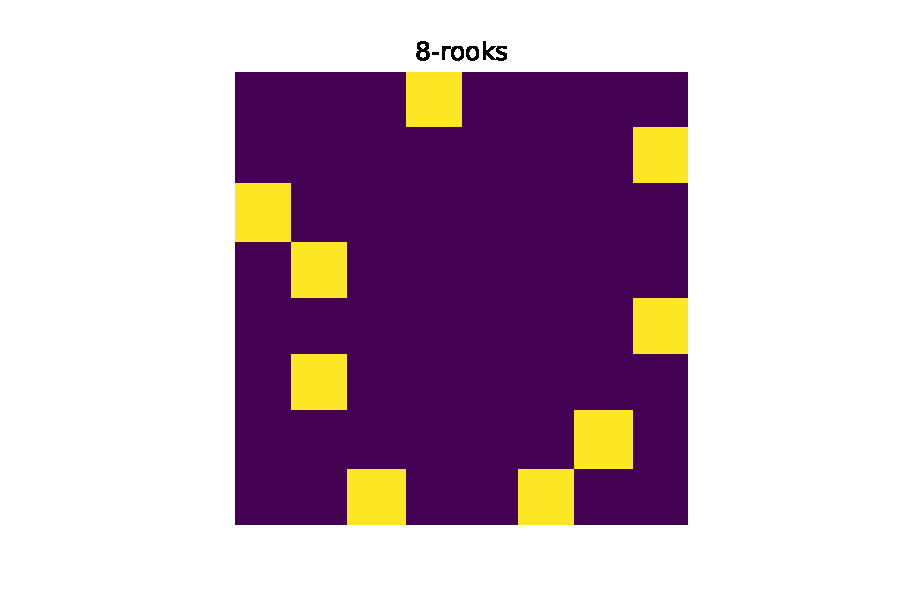
\includegraphics{Ex_03/Figures/8-rooks.pdf}
    \caption{Final state after 100 ansynchronus update steps.}
    \label{fig:my_label}
\end{figure}
\color{black}
\end{enumerate}





\subsection*{task 3.5 [20 points] \\[1ex] Hopfield nets: finding maximally different images}

Once again consider the matrix $\mat{X}$ of tiny images from task 3.3. However, let us simplify things and only consider the first $100$ of these images. Using numpy, we can accomplish this like so
\begin{python}
matX = matX[:,:100]
\end{python}

Given this truncated version of matrix $\mat{X}$, standardize the data it contains and store the result in a matrix $\mat{Y}$.

Next, given this new matrix $\mat{Y}$, compute a squared Euclidean distance matrix $\mat{D}^{n \times n}$ where, in our case $n=100$ and
\begin{equation*}
D_{ij} = \dsq{\vec{y}_i}{\vec{y}_j}.
\end{equation*}
If you do not know how to do this efficiently, you might want to consult
\begin{itemize}
\item[] C. Bauckhage, \href{https://www.researchgate.net/publication/266617010_NumPy_SciPy_Recipes_for_Data_Science_Squared_Euclidean_Distance_Matrices}{\textbf{``NumPy / SciPy Recipes for Data Science: Squared Euclidean Distance Matrices''}}, technical report, 2014 
\end{itemize}

\vspace{2cm}


Now, recall that, in exercise 01, we were concerned with the problem of finding $k$ data points that are as far apart as possible. Back then, we formalized this problem as follows
\begin{align*}
S^* = \amax{S \subset X} & \sum_{\vec{y}_i \in S} \sum_{\vec{y}_j \in S} \dsq{\vec{y}_i}{\vec{y}_j} \\
\st \; & \; \; \lvert S \rvert = k
\end{align*}

Working with the above distance matrix $\mat{D}$ and introducing a binary indicator vector $\vec{z} \in \{ 0, 1 \}^n$, this problem can also be cast as
\begin{equation}
\begin{aligned}
\vec{z}^* = \amax{\vec{z} \in \{ 0, 1 \}^n} & \; \trn{\vec{z}} \mat{D} \vec{z} \\
\st \; & \; \; \ipt{\vec{1}}{\vec{z}} = k
\end{aligned}
\tag{$\star$}
\end{equation}

This looks like a problem a Hopfield network could handle! So, go ahead and implement a Hopfield network that solves $(\star)$.

\textbf{Note:} $(\star)$ is written in terms of binary vectors $\vec{z}$. However, for the Hopfield networks we are interested in, we require problem formulations in terms of bipolar vectors $\vec{s}$. That is, you'll need to rewrite the problem in $(\star)$ as a QUBO that \textit{minimizes} over bipolar vectors (and make sure that the resulting weight matrix is hollow) before you implement the Hopfield net. (This is possible \ldots all you need to do is to be very careful and diligent with your algebraic manipulations).

Run your Hopfield net for several choices of $k$, say $k \in \{9, 16, 25\}$.

\textbf{Note:} Your Hopfield net will end up in a state $\vec{s} \in \{ -1, +1 \}^n$. \emph{If all goes well}, $k$ entries of $\vec{s}$ will have a value of $+1$ and the remaining $n-k$ entries will have a value of $-1$. The $+1$ entries of $\vec{s}$ will index $k$ maximally diverse columns of $\mat{Y}$. However, $\mat{Y}$ is a standardized version of $\mat{X}$. Hence, to visualize the outcome of your Hopfield network computations, use the resulting state vector $\vec{s}$ as an index into the columns of $\mat{X}$ and visualize the images you obtain this way.
%%%%%
%%%%%
%%%%% enter your plots here, i.e. replace "placeholder.pdf" by the name of the graphics files you created
%%%%%
%%%%%

\color{blue}

Lets first derive the weights of the hopfield network for this specific optimization problem.

Start by rewriting the initial quadratic program as follows
\begin{align*}
\Rightarrow \vec{z}^* = \amin{\vec{z} \in \{ 0, 1 \}^n} & \; -\trn{\vec{z}} \mat{D} \vec{z} \\
\st \; & \; \; (\ipt{\vec{1}}{\vec{z}} - k)^2 = 0
\end{align*}

Then convert from binary valued vectors to bipolar vectors using the isomorphic transformation $s = \frac12 (z+1)$
\begin{align*}
\Rightarrow \vec{s}^* = \amin{\vec{s} \in \{ -1, +1 \}^n} & \; -\frac14 \trn{\vec{(s+1)}} \mat{D} \vec{(s+1)} \\
\st \; & \; \; (\frac12 \ipt{\vec{1}}{\vec{(s+1)}} - k)^2 = 0
\end{align*}

\begin{align*}
    \trn{\vec{(s+1)}} \mat{D} \vec{(s+1)} &= \trn{\vec{s}} \mat{D} \vec{s} + 2 \cdot \trn{\vec{1}} \mat{D} \vec{s} \textcolor{gray}{ + \trn{\vec{1}} \mat{D} \vec{1}} \\
    \frac12 \ipt{\vec{1}}{\vec{(s+1)}} - k &= \frac12 (\ipt{\vec{1}}{\vec{s}} + \ipt{\vec{1}}{\vec{1}}) - k \\
        &= \frac12 (\ipt{\vec{1}}{\vec{s}} + n - 2 k) \\
        &= \frac12 (\ipt{\vec{1}}{\vec{s}} + c) \;\;\;\text{for $c = n - 2k$}
\end{align*}

$$
\begin{aligned}
\Rightarrow \vec{s}^* = \amin{\vec{s} \in \{ -1, +1 \}^n} & \; -\frac14 \trn{\vec{s}} \mat{D} \vec{s} - \frac12 \cdot \trn{\vec{1}} \mat{D} \vec{s} \\
\st \; & \; \; \frac14 (\ipt{\vec{1}}{\vec{s}} + c)^2 = 0
\end{aligned}
$$

Now using Lagrange-Multipliers this can be rewritten as an unconstraint optimization problem

\begin{align*}
    \Rightarrow L(s, \lambda) &= -\frac14 \trn{\vec{s}} \mat{D} \vec{s} - \frac12 \cdot \trn{\vec{1}} \mat{D} \vec{s} + \frac14 \lambda (\ipt{\vec{1}}{\vec{s}} + c)^2 \\
    &= -\frac14 \trn{\vec{s}} \mat{D} \vec{s} - \frac12 \cdot \trn{\vec{1}} \mat{D} \vec{s} + \frac14 \lambda (\ipt{\vec{s}}{\vec{1}}\ipt{\vec{1}}{\vec{s}} + 2c\ipt{\vec{1}}{\vec{s}} + c^2) \\
    &= \frac14 \trn{\vec{s}} (\lambda\vec{1}\trn{\vec{1}} -\mat{D}) \vec{s} + \frac12 \cdot (\lambda c\trn{\vec{1}} - \trn{\vec{1}} \mat{D}) \vec{s} + \frac14 \lambda c^2 \\
    &= \frac14 \trn{\vec{s}} (\lambda\vec{1}\trn{\vec{1}} -\mat{D}) \vec{s} + \frac12 \cdot \trn{(\lambda c\vec{1} - \trn{\vec{D}} \mat{1})} \vec{s} + \frac14 \lambda c^2 \\
\end{align*}

Lastly the coefficient matrix needs to be hollow, which can be achived as follows

\begin{align*}
    \Rightarrow L(s, \lambda) &= \frac14 \trn{\vec{s}} (\lambda\vec{1}\trn{\vec{1}} - \mat{D} -\lambda \mat{I}) \vec{s} + \trn{\vec{s}} \lambda\mat{I} \vec{s} + \frac12 \cdot \trn{(\lambda c\vec{1} - \trn{\vec{D}} \mat{1})} \vec{s} + \frac14 \lambda c^2 \\
    &= \frac14 \trn{\vec{s}} (\lambda\vec{1}\trn{\vec{1}} - \mat{D} -\lambda \mat{I}) \vec{s} + \frac12 \cdot \trn{(\lambda c\vec{1} - \trn{\vec{D}} \mat{1})} \vec{s} + \textcolor{gray}{\lambda n + \frac14 \lambda c^2}
\end{align*}

Note that the distance matrix $\mat{D}$ is already hollow by definition.

This final form of the optimization problem can be directly optimized using a hopfield network with
\begin{align*}
    \mat{W} &= -\frac12(\lambda \mat{1}\trn{\mat{1}} - D - \lambda \mat{I}) \\
    \vec{\theta} &= \frac12(\lambda c \vec{1} - \ipt{\mat{D}}{\vec{1}}) \\
    \\
    \Rightarrow s^* &= \amin{\vec{s} \in \{ -1, +1 \}^n} -\frac12 \trn{\vec{s}}\mat{W}\vec{s} + \trn{\vec{\theta}}\vec{s}
\end{align*}

\color{black}
\begin{python}
# load and preprocess data
X = np.load('Data/faceMatrix.npy').astype('float')
X = X[:, :100]
Y = X - X.mean(axis=-1, keepdims=True)
# also convert the data matrix to the actual image
# layout for easier visualization later on
imgs = X.reshape(19, 19, -1).transpose(2, 0, 1)

# compute the distance matrix using method 5 from
# "NumPy/SciPy Recipes for Data Science:Squared Euclidean Distance Matrices"
def squared_EDM(X:np.ndarray):
    m, n = X.shape
    # compute gram matrix
    G = X.T @ X
    # compute matrix H
    H = np.tile(np.diag(G), (n, 1))
    return H + H.T - 2*G
D = np.sqrt(squared_EDM(Y))

def maximally_different(
    D:np.ndarray, 
    k:int, 
    lam:float =7000     # we handpicked lambda by try and error :)
):
    # get the number of objects to choose from
    n = D.shape[0]
    # build hopfield network parameters that were derived above
    W = -0.5 * (np.full((n, n), lam) - lam * np.eye(n) - D)
    theta = 0.5 * (np.full(n, lam * (n - 2*k)) - D.sum(axis=-1))
    # create an initial state
    s = np.ones(n)
    
    # apply hopfield optimization
    s = hopfield_run_async(s, W, theta, tmax=100_000)
    # create mask indicating maximally different objects
    return (s == 1.0)

# helper function for easily visualization
# of the found candidates
def show_maximally_different(
    imgs:np.ndarray, 
    D:np.ndarray, 
    k:int
):
    mask = maximally_different(D, k=k)
    imgs = imgs[mask, ...]
    print(mask.sum())
    assert mask.sum() >= k
    # visualize
    n, m = ceil(np.sqrt(k)), int(np.sqrt(k))
    fig, axs = plt.subplots(n, m)
    for i, ax in enumerate(axs.flatten()):
        ax.axis('off')
        ax.imshow(imgs[i, ...], cmap='gray')
    # return the figure
    return fig
    
# create the plots for k = 9, 16, 25
fig = show_maximally_different(imgs, D, k=9)
fig.savefig("Figures/imgs_k9.pdf")
fig = show_maximally_different(imgs, D, k=16)
fig.savefig("Figures/imgs_k16.pdf")
fig = show_maximally_different(imgs, D, k=25)
fig.savefig("Figures/imgs_k25.pdf")

\end{python}

\begin{center}
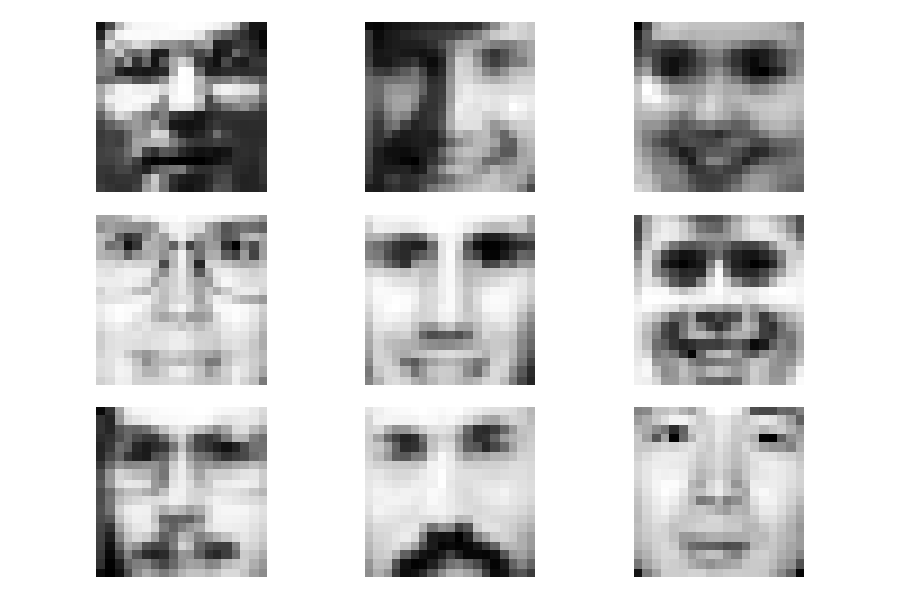
\includegraphics[width=0.32\textwidth]{Ex_03/Figures/imgs_k9.pdf}
\hfill
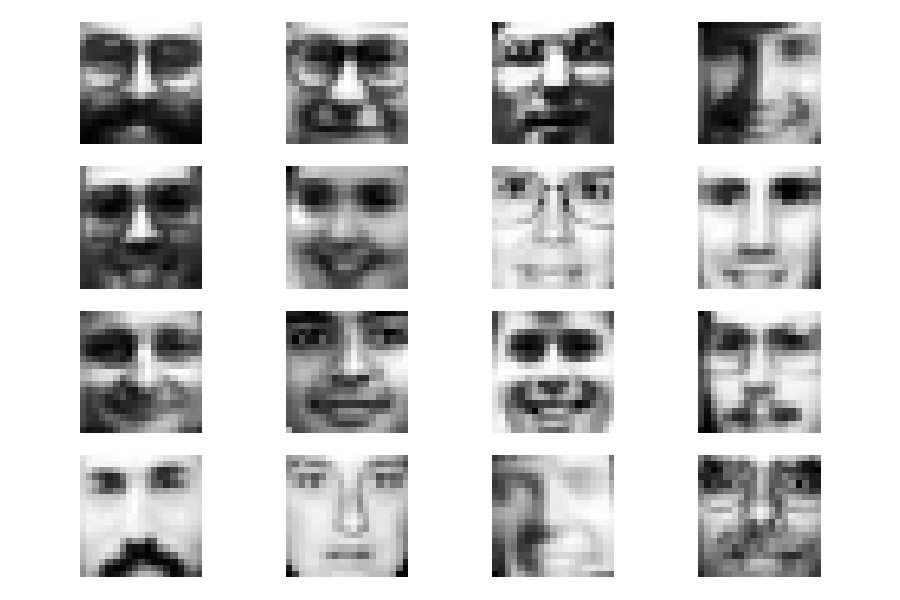
\includegraphics[width=0.32\textwidth]{Ex_03/Figures/imgs_k16.pdf}
\hfill
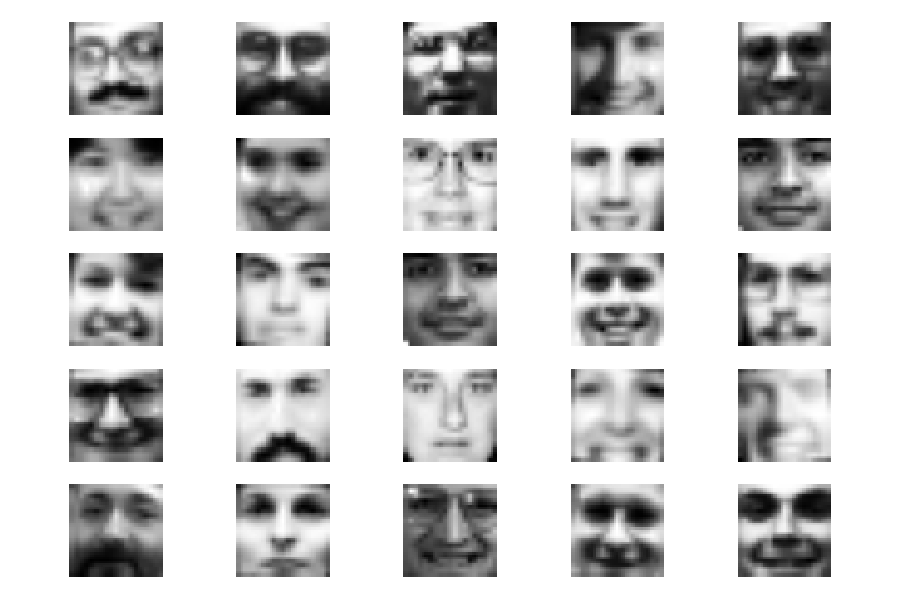
\includegraphics[width=0.32\textwidth]{Ex_03/Figures/imgs_k25.pdf}
\end{center}
%%%%%
%%%%%
%%%%%
%%%%%
%%%%%





\end{document}
